%CHKTEX-FILE 46

\subsection*{FRIDA Hardware Description}
\label{sec:annex-OPL}
% In this section briefly describe the software and hardware of the robot

\setlength\intextsep{0pt}
\begin{wrapfigure}[10]{h}{0.33\textwidth}
	\centering
	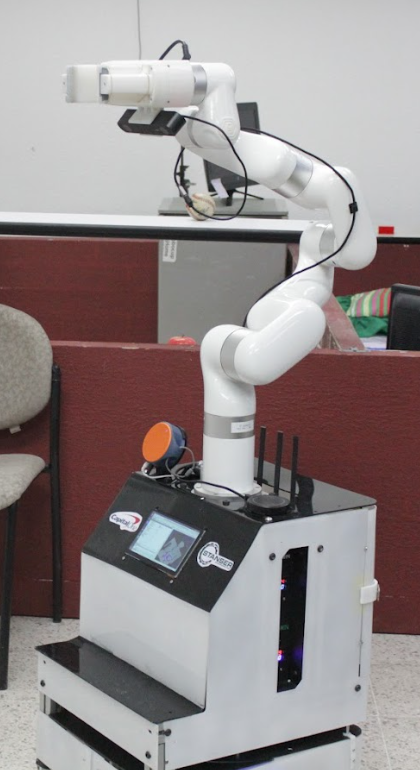
\includegraphics[width=0.3\textwidth]{TDPTemplate-master/images/frida.png}
	\caption{FRIDA}%
	\label{fig:frida}
\end{wrapfigure}

\begin{itemize}
	\item Base: A modified EAI Dashgo B1 differential drive robot was used for mobility purposes and motors with encoders for odometry purposes.
	\item Computers: NVIDIA Jetson AGX Orin 64GB.
	\item Batteries: A total of three 24v li-ion batteries are used, one for the xArm, Jetson Orin and Dashgo.
	\item Manipulator: xArm 6.
    \item Gripper: 2 finger parallel custom 3D printed gripper with force resistive sensors on each finger and an IR sensor for detecting objects in front of it. It uses an ESP32 as the microcontroller.
	\item Vision: Stereolabs ZED2 camera attached to the EOF of the xArm that runs the vision tasks and transmits data through a USB cable to the Jetson Orin.
        \item HRI: Seed Studio ReSpeaker Microphone array, Logitech X100 Wireless Portable Speaker, and a HDMI LCD touch screen 7" display.
        \item Navigation: RP Lidar A1.
        \item Base cover: Custom acrylic manufactured structure to protect and secure the interior electronics and components.
	\item Robot dimensions: Height 180 cm (fully extended), base footprint 50 cm $\times$ 42 cm
	\item Robot weight: 40 kg.
\end{itemize}

\subsection*{FRIDA Software Description}

\begin{itemize}
	\item Platform: ROS 2, Jazzy distribution.
    \item Integration: Docker
	\item Navigation: ROS 2 Navigation Stack, RTAB-Map
	\item Person analysis: Torch, InsightFace, YOLO11-pose, MediaPipe, ByteTrack, Moondream2
	\item Speech recognition: WhisperLive with faster-whisper
    \item Keyword spotting: Open Wake Word
	\item Text processing: Llama 3.2, sentence-transformers/ all-MiniLM-L6-v2
    \item Text To Speech: Kokoro-82M
	\item Object detection: GroundingDINO, SAM 3, YOLO11, YOLOE, DINOv2
    \item Manipulation planning: MoveIt 2, GPD
    \item Point cloud processing: PCL, RANSAC
\end{itemize}
